% LaTeX.tex
% Example of PROCEEDINGS PAPER of the 26th ABCM International Congress of Mechanical Engineering
% COBEM 2021 - ONLINE
% Based on the templates of COBEM2015, COBEM2017, and COBEM2019

\documentclass[10pt,fleqn,a4paper,twoside]{article}
\usepackage{abcm}
\usepackage{amsmath}
\usepackage{tikz}
\usepackage{float}
\usepackage{tikz}
\usetikzlibrary{patterns}
\usepackage{relsize}
\usetikzlibrary{shapes,arrows,arrows.meta,matrix}


\def\shortauthor{L. Marques}
\def\shorttitle{A Blood Flow Numerical Simulation using ALE-FE Method for 2D Navier-Stokes Equation}



\begin{document}
\fphead
\hspace*{-2.5mm}\begin{tabular}{||p{\textwidth}}
\begin{center}
\vspace{-4mm}
\title{ 
BLOOD FLOW NUMERICAL SIMULATION USING ALE-FE METHOD FOR 2D NAVIER-STOKES EQUATION} 
%
\end{center}
\authors{Leandro Marques} \\
\institution{COPPE/Federal University of Rio de Janeiro - UFRJ, R. Horacio Macedo, 2030, Rio de Janeiro, Brazil}\\
\institution{marquesleandro.uerj@gmail.com} \\
\\
\abstract{\textbf{Abstract.} 
The present work aims at developing a computational framework to simulate the drug diffusion in the bloodstream in a coronary artery 
with drug-eluting stent implanted.
The blood was modeled as a single-phase, incompressible 
and Newtonian fluid 
and the Navier-Stokes equation was approximated 
according to the Finite Element Method (FEM) in an
Arbitrary Lagrangian-Eulerian (ALE) description.
The dynamics of drug-eluting concentration in
bloodstream was investigated using 
the drug-eluting stent
in microchannels with with atherosclerosis.
The results reveal the possibility of other simulations
using complex geometries.
}

}
\\
\\
\keywords{\textbf{Keywords:} Navier-Stokes; Finite Element Method; Semi-Lagrangian; Drug-Eluting Stent; Arbitrary Lagrangian-Eulerian.}\\
\end{tabular}

\section{INTRODUCTION}

According to the World Health Organization (WHO) \cite{oms2018},
cardiovascular diseases have remained the leading
death causes globally in the last 15 years. 
It is estimated that \mbox{15.2 million} people died from CVD in 2016,
representing 26.7\% of all deaths in the world. 
In Brazil, about 38\% of deaths due to CVD is in the procutive age range
(18 to 65 years) and the estimated
costs of CVD were R\$ 37.1 billion
in 2015, that is, 0.7\% GDP \cite{siqueira2017}.
About 60\% of CVD deaths
occurred due to coronary artery disease (CAD).
The main cause of CAD is the atherosclerosis which consists of
the accumulation of fat plaques inside the artery wall causing
a decrease in lumen diameter.
The Atherosclerosis can be prevented with a change in harmful habits
such as: cigarette smoking, physical inactivity/low fitness and poor dietary habits \cite{spring2013}.
For a corrective approach, however, two treatments can be performed:
the \textit{Coronary Artery Bypass Graft} (CABG) or a 
procedure minimally invasive called 
\textit{Percutaneous Transluminal Coronary Angioplasty} (PTCA)
\cite{gruntzig1979},
where a wire tube (\textit{stent}) is placed.

\smallskip
In 2001,
Hwang, Wu and Edelman \cite{hwang2001} presented
a numerical simulation in a coronary artery, 
where the stent strut 
was coated with the drug.
Such procedure proved to be a promising option
for the treatment of atherosclerosis and reestonosis.
This new type of stent
would be known as \textit{drug-eluting stent}.
In the following years,
\mbox{Zunino et al. \cite{zunino2009}} presented 
in 2009 a complete overview
of mathematical models and finite element numerical simulation
applied to the  modeling of drug eluting stens and
of their interaction with
the coronary arteries, take into account the stent expansion,
fluid dynamics around the stent and drug release. The numerical
simulation showing recirculation zones downstream
has important consequences on the drug release process.
The authors concluded that the drug released into the lumem
does not significantly contribute to the permanent drug
deposition into the arterial wall and only an small fraction of
the total amount drug stored into the stent was effectively
delivered to the artery.
In 2018, Lucena et al. \cite{lucena2018} presented
the simulation of the transport of the drug \textit{sirolimus}
 on the wall of an artery modeled as a porous and anisotropic medium.
 The authors estimated that
 about 47\% of the drug is diffused in the lumen and it is lost in
 the bloodstream. The spatial distribution of the drug, however,
 is greatly influenced by blood flow and the properties of
the artery wall. Thus, such results are susceptible to the
 patient health conditions.
In the following years,
Marques and Anjos \cite{marques2021} presented the
a numerical study on the drug diffusion in the bloodstream
in a coronary artery with drug-eluting stent implanted,
using the streamfunction-vorticity formulation.
The atherosclerosis has a direct influence
on the drug-eluting concentration field, 
modifying the dynamics of the drug diffusion in
the bloodstream and the horizontal velocity reaches
three times the blood velocity in coronary artery 
without atherosclerosis.
Therefore, we propose the development of a numerical code 
using an ALE-FE method for 2D Navier-Stokes Equation
with the drug diffusion in bloodstream.

\medskip
The dynamics of concentration diffusion in coronary arteries 
requires a robust numerical method to compute the solution 
of the differential equations in a relevant model,
especially due to the thin concentration boundary layer 
in the vicinity of the implanted
stents that must be accurately capture. 
The equations that govern the dynamics of blood
flow in a coronary artery were developed according 
to continuum media assumption. Thus,
the universal conservation laws such as mass, momentum 
and species transport were used
in an Arbitrary Lagrangian-Eulerian context. 
The blood was modeled as single-phase, incompressible, Newtonian
and a diffusion coefficient were taken under consideration 
to evaluate different drug
transport alongside the blood flow. 
Thus, the Navier--Stokes equation is presented 
with drug-eluting transport equation using
the Finite Element method. 
The domain was discretized on an unstructured mesh using the
GMSH open source software, 
where the triangular element with linear interpolation
was used for pressure field and with cubic interpolation
was used for velocity and concentration fields.
Therefore, the Babuska-Brezzi \cite{babuska1971}\cite{brezzi1974} 
was
satisfied. 
The equations were discretized in spatial domain using the Galerkin formulation
and in temporal domain the semi-Lagrangian scheme 
was used to discretized the material
derivative using first order backward difference scheme. 
The computational code was
developed in Python Language using the Object-Oriented Paradigm (OPP) 
and the linear
system of equations that comes from implementing the FEM is 
solved through direct solver available in the public 
library for scientific tools SciPy, using the sparse matrices.


\smallskip
The dynamics of
concentration diffusion in a coronary artery with 
drug-eluting stent was investigated in
a complex geometry, using a two-dimensional approach. 
That is, the coronary artery
was approximated as a plannar domain. 
Due to symmetry of problem, only half domain
was simulated. 
The case is called the \textit{Curved Channel with Stent}, 
where this geometry is a model of the real coronary artery and 
an atherosclerosis was considered using a sinusoidal
equation to model 40\% of channel obstruction.
The concentration diffusion was investigated using 
a drug concentration diffusity, 
whose \textit{Schmidt numbers} $Sc$
was: $Sc = 1$, which are equivalent to drug-lumen 
mass diffusion rate of
$D = 3$$\times$10$^{−6}$ m$^{2}/s$ respectively.


\section{MATHEMATICAL MODEL}
The dynamics of concentration diffusion in coronary 
arteries require a robust numerical method to compute 
the solution of the differential equations in a relevant model. The
equations that govern the dynamics of blood flow in a 
coronary artery were developed
according to continuum media assumption. 
Thus, the universal conservation laws such as
mass, momentum and species transport were used in an 
Arbritary Lagragian-Eulerian context. The blood was
modeled as single-phase, incompressible, 
Newtonian and a drug diffusion coefficient
was taken under consideration to evaluate 
the drug transport alongside the blood flow.
The Navier-Stokes equation is shown with 
species transport equation in a 2-dimensional approach: 

\begin{align}
& \nabla \cdot \textbf{v} 
= 0 \label{continuity}
\\[10pt] 
& \frac{D \textbf{v}}{D t} 
 =
 - \nabla p
 + \frac{1}{Re} \nabla^{2} \textbf{v} \label{vorticity}
 \\[10pt] 
& \frac{D e}{D t} 
 =
 \frac{1}{ReSc} \nabla^{2} e \label{especie quimica}
\end{align}


\noindent
where, 
\textbf{v} is the material velocity field,
\textit{p} is the pressure field,
\textit{e} is the concentration field,
\textit{D/Dt} is the material derivative,
\textit{Re} $= \rho u$R/$\mu$ is the Reynolds number,
where $\rho$ is the blood density (kg/m$^{3}$),
$u$ is the blood velocity in the coronary artery (m/s),
$R$ is the lumen radius of the coronary artery (m)
and $\mu$ is the blood viscosity (N.s/m$^{2}$),
\textit{Sc} $= \mu / \rho D$ is the Schmidt number,
where $D$ is the mass diffusion rate of the drug (m$^{2}$/s) and
\textit{x} and \textit{y} are the spatial variables.


\bigskip
\noindent
The boundaries conditions used were:

\begin{itemize}
\item {\textit{inflow condition}:
 this condition was specified in the left line of the geometries in
 this work, where an mass inflow is desired.
 For such a condition, $u = u_{o}$
 and $v = v_{o}$, where $u_{o}=1.5[1-(y/R)^{2}]$ and $y_{o}=0$}
 \item {\textit{wall condition}:
 this condition is specified at wall boundary, that is,
 the top line of the geometries in this work, where
 the no-slip condition is set.
 All the velocity components are specified with
 null values.}
 \item {\textit{outflow condition}:
 this condition represents a state where is close to a
 fully developed profile, that is, the right line of the
 geometries in this work.
 No prescribed value is specified for the velocity field
 and the pressure field is set the null value.}
 \item {\textit{free-slip condition (symmetry)}:
 this condition is specified at the symmetric axis,
 that is, the bottom line of the geometries in this work.
 The vertical velocity component is null and the derivative of
 the horizontal component is also null value.}
 \item {\textit{strut condition (semi-circles)}:
 this condition is used on the semi-circles of drug-eluting stent.
 The vertical and horizontal
 velocity components are specified with null value.
 The concentration field is specified as $e=e_{o}$, where $e_{o}=1$.}
\end{itemize}


To solve these governing equations, a numerical method is necessary. In this work, the
Finite Element Method was used to approximate the differential equations.
The domain was discretized on an unstructured mesh using the
GMSH open source software, 
where the triangular element with linear interpolation
was used for pressure field and with cubic interpolation
was used for velocity and concentration fields.
Therefore, the Babuska-Brezzi \cite{babuska1971}\cite{brezzi1974} 
was
satisfied. 
The equations were discretized in spatial domain using the Galerkin formulation.
Thus, we present the semi-discrete
matricial form of the Navier--Stokes using the Galerkin method
as follows:


\vspace{-0.4cm}
\begin{equation}
 D\textbf{v} = 0
\end{equation}

\vspace{-0.65cm}
\begin{equation}
 M \frac{D \textbf{v}}{Dt} 
 + \frac{1}{\textit{Re}} K \textbf{v}
 - Gp
 = 0 \label{vorticity matrix}
\end{equation}

\vspace{-0.65cm}
\begin{equation}
 M \frac{De}{Dt} 
 + \frac{1}{\textit{ReSc}} K e
 = 0 \label{concentration matrix}
\end{equation}



\noindent
where,
\textit{M} is mass matrix,
\textit{D} is divergent matrix,
\textit{G} is gradient matrix and
\textit{K} is stiffness matrix.
In this moment, 
the velicity $\textbf{v}$,
the pressure $p$ and
the drug concentration field $e$ field
are discretized in the spatial domain but
continuos in the temporal domain.
Then, for time discretization, the semi-Lagrangian Method was used. 
This method was proposed by Sawyer in 1963 \cite{sawyer1963} for atmospheric flow numerical simulation using vorticity-advection equation, allowing to use large time steps without numerical instability. 
However, because of a limited computer capability, the use of such methodology to model several fluid flow problems, with high order differences and fine mesh, came later in the 1980s through the work of Robert \cite{robert1981} and Pironneu \cite{pironneau1982}, where the semi-lagrangian scheme would be able to run models faster than the Eulerian scheme, besides being unconditionally stable and only symmetric linear systems to solve. 
Therefore the semi-lagrangian method discretized and 
computed the material derivative along the trajectory 


\vspace{-0.4cm}
\begin{equation}
 \frac{D \textbf{v}}{D t} \approx
 \frac{\textbf{v}_{i}^{n+1} - \textbf{v}_{d}^{n}}{\Delta t}
\end{equation}

\noindent
where, 
$D\textbf{v}/Dt$ is material derivative of $\textbf{v}$ and
the right-hand side equation is material derivative discretized using first order backward difference scheme.
The variable $t$ is time, 
$\textbf{v}_{i}^{n+1}$ is the velocity field calculated in current time step at the current node position and
$\textbf{v}_{d}^{n}$ is the velocity field calculated in previous time step at the departure node position.
The departure node is found by solving equation $\mathbf{x}_{d}^{n} = \mathbf{x}_{i}^{n+1} - \mathbf{v} \Delta t$, using the initial condition $\mathbf{x}_{i}^{n+1} = \mathbf{x}(t^{n+1})$ as shown in Figure \ref{semi-lagrangian figure}a . 
A algorithm must be used to find the element that the departure node be, then the velocity field in departure node ($\textbf{v}_{d}^{n}$) is calculed by barycenter coordinates interpolation between nodes of element found.
As shown in Figure \ref{semi-lagrangian figure}b , three situations may occur depending on the trajectory: the first and the second situations are similar, differentiating only the trajectory length. 
In the first situation, the departure node is inside near element from current node, while the second situation the departure node is inside far element from current node. 
The third situation, the departure node is outside domain then the vorticity field in departure node receives the boundary condition value of nearest node to departure node.

\vspace{-0.5cm}
\begin{figure}[H]
\begin{center}
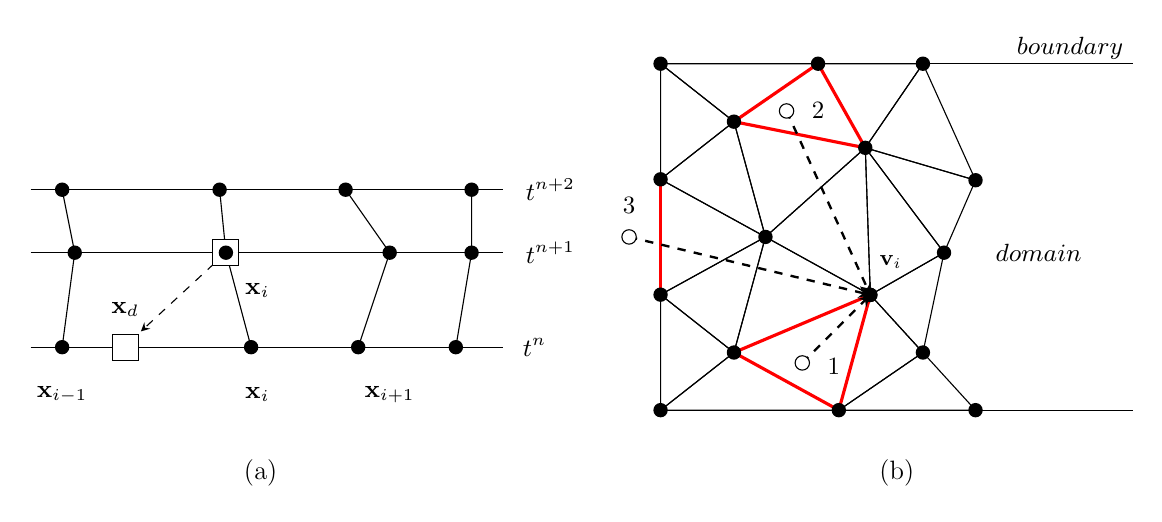
\begin{tikzpicture}[scale=4]

 % FIGURE A
 % grid
 \draw (0.5,0.7) -- (2.0,0.7);
 \draw (0.5,1.0) -- (2.0,1.0);
 \draw (0.5,1.2) -- (2.0,1.2);

 \draw (0.60,0.7) -- (0.64,1.0) -- (0.60,1.2);
 \draw (1.20,0.7) -- (1.12,1.0) -- (1.10,1.2);
 \draw (1.54,0.7) -- (1.64,1.0) -- (1.50,1.2);
 \draw (1.85,0.7) -- (1.90,1.0) -- (1.90,1.2);



 % material points
 \draw[dashed,-stealth] (1.12,1.0) -- (0.85,0.75);
 \node[rectangle, fill=white, draw, inner sep=0pt, minimum size=9.4pt] at (0.8,0.7) {};
 \node[rectangle, fill=white, draw, inner sep=0pt, minimum size=9.4pt] at (1.12,1.0) {};
 

 % nodes
 \node[circle, fill=black, inner sep=0pt, minimum size=5.2pt] at (0.60,0.7) {};
 \node[circle, fill=black, inner sep=0pt, minimum size=5.2pt] at (1.20,0.7) {};
 \node[circle, fill=black, inner sep=0pt, minimum size=5.2pt] at (1.54,0.7) {};
 \node[circle, fill=black, inner sep=0pt, minimum size=5.2pt] at (1.85,0.7) {};

 \node[circle, fill=black, inner sep=0pt, minimum size=5.2pt] at (0.64,1.0) {};
 \node[circle, fill=black, inner sep=0pt, minimum size=5.2pt] at (1.12,1.0) {};
 \node[circle, fill=black, inner sep=0pt, minimum size=5.2pt] at (1.64,1.0) {};
 \node[circle, fill=black, inner sep=0pt, minimum size=5.2pt] at (1.90,1.0) {};

 \node[circle, fill=black, inner sep=0pt, minimum size=5.2pt] at (0.60,1.2) {};
 \node[circle, fill=black, inner sep=0pt, minimum size=5.2pt] at (1.10,1.2) {};
 \node[circle, fill=black, inner sep=0pt, minimum size=5.2pt] at (1.50,1.2) {};
 \node[circle, fill=black, inner sep=0pt, minimum size=5.2pt] at (1.90,1.2) {};


 % legend
 \node[draw=none, scale=1.0] at (0.80,0.82) {\small $\mathbf{x}_{d}$};
 \node[draw=none, scale=1.0] at (1.22,0.88) {\small $\mathbf{x}_{i}$};

 \node[draw=none, scale=1.0] at (2.10,0.70) {\small $t^{n}$};
 \node[draw=none, scale=1.0] at (2.15,1.00) {\small $t^{n+1}$};
 \node[draw=none, scale=1.0] at (2.15,1.20) {\small $t^{n+2}$};

 \node[draw=none, scale=1.0] at (0.60,0.55) {\small $\mathbf{x}_{i-1}$};
 \node[draw=none, scale=1.0] at (1.22,0.55) {\small $\mathbf{x}_{i}$};
 \node[draw=none, scale=1.0] at (1.64,0.55) {\small $\mathbf{x}_{i+1}$};


 % -------------------------------------------------------------------
 % FIGURE B
 % boundary 
 \draw (2.5,1.6) -- (4.0,1.6);
 \draw (2.5,1.6) -- (2.5,0.5);
 \draw (2.5,0.5) -- (4.0,0.5);

 % nodes
 \coordinate (A) at (2.500,0.5000) {};
 \coordinate (B) at (2.500,0.8667) {};
 \coordinate (C) at (2.500,1.2330) {};
 \coordinate (D) at (2.500,1.6000) {};
 \coordinate (E) at (2.733,0.6830) {};
 \coordinate (F) at (2.833,1.0500) {};
 \coordinate (G) at (2.733,1.4160) {};
 \coordinate (H) at (3.000,1.6000) {};
 \coordinate (I) at (3.066,0.5000) {};
 \coordinate (J) at (3.166,0.8660) {};
 \coordinate (K) at (3.150,1.3330) {};
 \coordinate (L) at (3.333,1.6000) {};
 \coordinate (M) at (3.500,0.5000) {};
 \coordinate (N) at (3.333,0.6830) {};
 \coordinate (O) at (3.400,1.0000) {};
 \coordinate (P) at (3.500,1.2300) {};

 % elements
 \draw (A) -- (E) -- (B) -- cycle;
 \draw (A) -- (I) -- (E) -- cycle;
 \draw (E) -- (J) -- (F) -- cycle;
 \draw (E) -- (F) -- (B) -- cycle;
 \draw (B) -- (F) -- (C) -- cycle;
 \draw (J) -- (K) -- (F) -- cycle;
 \draw (F) -- (K) -- (G) -- cycle;
 \draw (C) -- (F) -- (G) -- cycle;
 \draw (C) -- (G) -- (D) -- cycle;
 \draw (G) -- (H) -- (D) -- cycle;
 \draw (I) -- (N) -- (J) -- cycle;
 \draw (I) -- (M) -- (N) -- cycle;
 \draw (N) -- (O) -- (J) -- cycle;
 \draw (J) -- (O) -- (K) -- cycle;
 \draw (P) -- (L) -- (K) -- cycle;
 \draw (K) -- (L) -- (H) -- cycle;
 \draw (O) -- (P) -- (K) -- cycle;
 \draw[red,line width=0.04cm] (I) -- (J) -- (E) -- cycle;
 \draw[red,line width=0.04cm] (B) -- (C);
 \draw[red,line width=0.04cm] (G) -- (K) -- (H) -- cycle;
 

 % draw nodes
 \node[circle, fill=black, inner sep=0pt, minimum size=5.2pt] at (A) {};
 \node[circle, fill=black, inner sep=0pt, minimum size=5.2pt] at (B) {};
 \node[circle, fill=black, inner sep=0pt, minimum size=5.2pt] at (C) {};
 \node[circle, fill=black, inner sep=0pt, minimum size=5.2pt] at (D) {};
 \node[circle, fill=black, inner sep=0pt, minimum size=5.2pt] at (E) {};
 \node[circle, fill=black, inner sep=0pt, minimum size=5.2pt] at (F) {};
 \node[circle, fill=black, inner sep=0pt, minimum size=5.2pt] at (G) {};
 \node[circle, fill=black, inner sep=0pt, minimum size=5.2pt] at (H) {};
 \node[circle, fill=black, inner sep=0pt, minimum size=5.2pt] at (I) {};
 \node[circle, fill=black, inner sep=0pt, minimum size=5.2pt] at (J) {};
 \node[circle, fill=black, inner sep=0pt, minimum size=5.2pt] at (K) {};
 \node[circle, fill=black, inner sep=0pt, minimum size=5.2pt] at (L) {};
 \node[circle, fill=black, inner sep=0pt, minimum size=5.2pt] at (M) {};
 \node[circle, fill=black, inner sep=0pt, minimum size=5.2pt] at (N) {};
 \node[circle, fill=black, inner sep=0pt, minimum size=5.2pt] at (O) {};
 \node[circle, fill=black, inner sep=0pt, minimum size=5.2pt] at (P) {};


 % arrow
 \draw[dashed,line width=0.03cm,-stealth]  (2.95,0.65) -- (J) ;
 \draw[dashed,line width=0.03cm,-stealth]  (2.90,1.45) -- (J) ;
 \draw[dashed,line width=0.03cm,-stealth]  (2.4,1.05)  -- (J) ;

 \node[circle, fill=black, inner sep=0pt, minimum size=5.2pt] at (J) {};

 % departure nodes
 \node[circle, fill=white, draw, inner sep=0pt, minimum size=5.2pt] at (2.95,0.65) {};
 \node[circle, fill=white, draw, inner sep=0pt, minimum size=5.2pt] at (2.90,1.45) {};
 \node[circle, fill=white, draw, inner sep=0pt, minimum size=5.2pt] at (2.4,1.05) {};


 
 % legend
 \node[draw=none, scale=0.9] at (3.23,0.97) {\small $\textbf{v}_{i}$};
 
 \node[draw=none, scale=0.9] at (3.05,0.64) {$1$};
 \node[draw=none, scale=0.9] at (3.00,1.45) {$2$};
 \node[draw=none, scale=0.9] at (2.4,1.15) {$3$};

 \node[draw=none, scale=1.0] at (3.7,1.0) {\small $domain$};
 \node[draw=none, scale=1.0] at (3.8,1.65) {\small $boundary$};



 \node[draw=none, scale=0.8] at (1.23,0.3) {\large (a)};
 \node[draw=none, scale=0.8] at (3.25,0.3) {\large (b)};

\end{tikzpicture}
\end{center}
\caption{In (a), an one-dimensional space scheme
 where the departure node $x_{d}$ is found by integrating the 
mesh backward time. In (b), a two-dimensional space scheme
where three situations may occur in searching procedure.}
\label{semi-lagrangian figure}
\end{figure}

\medskip
The triangular element with linear interpolation was used
for the pressure field and a modified cubic element 
(2D MINI) was used
for the velocity field, 
in order to respect the Babuska-Brezzi restriction
\cite{babuska1971}\cite{brezzi1974}.
These elements consists in three nodes in the vertices
and one node in the baricentric for MINI element case.
The elementary matrices of 
this element are calculated using the Gaussian Quadrature, 
whose parameters can be found in the literature \cite{cowper1973}. 
\hl{This element is represented by the Figure} \ref{fig:element},
\noindent
where
a linear combination of the area
coordinates
$L_1$,
$L_2$ and
$L_3$
generates the cubic shape functions
$N_1$ to $N_4$.
The velocity $\textbf{v}$ and
concentration $e$ fields
are evaluated and computed at all nodes, whereas
the pressure field $p$ is computed at vertices nodes; 

\begin{figure}[H]
\begin{center}
\vspace{-0.5cm}
\begin{tikzpicture}[scale=3] 
 \draw (0,0) -- (1,0) -- (0.5,1) -- cycle;
 \node[circle, fill=black, inner sep=0pt, minimum size=5pt,label=below left:{1}] at (0,0) {};
 \node[circle, fill=black, inner sep=0pt, minimum size=5pt,label=below right:{2}] at (1,0) {};
 \node[circle, fill=black, inner sep=0pt, minimum size=5pt,label=above:{3}] at (0.5,1) {};
 \node[circle, fill=black, inner sep=0pt, minimum size=5pt,label=below:{4}] at (0.5,0.33) {};
 \node[draw, circle, thick, minimum size=7pt,label=below left:{}] at (0,0) {};
 \node[draw, circle, thick, minimum size=7pt,label=below left:{}] at (1,0) {};
 \node[draw, circle, thick, minimum size=7pt,label=below left:{}] at (0.5,1) {};

 \node[circle, fill=black, inner sep=0pt, minimum size=5pt,label=right left:{velocity nodes}] at (1.5,0.5) {};
 \node[circle, fill=black, inner sep=0pt, minimum size=5pt,label=right left:{concentration nodes}] at (1.5,0.7) {};
 \node[circle, draw, thick, inner sep=0pt, minimum size=7pt,label=right left:{pressure nodes}] at (1.5,0.3) {};

 \node[draw=none, align=left, scale=1.2] at (3.2,0.4)
                                               {$N_1 = L_1 - 9L_1L_2L_3$\\
                                                $N_2 = L_2 - 9L_1L_2L_3$\\
                                                $N_3 = L_3 - 9L_1L_2L_3$\\
                                                $N_4 = 27L_1L_2L_3$};



\end{tikzpicture}
\end{center}
\caption{
The linear triangle finite element
for pressure field and
the MINI element for velocity field.
The
$L_1$,
$L_2$ and
$L_3$
are the linear combination
of the triangle area
coordinates and
$N_1$,
$N_2$,
$N_3$ and
$N_4$
are the resulting shape functions.
}
\label{fig:element}
\end{figure}

\smallskip
Thus, we present the final version of the discrete matrix form of the dimensionless
governing equations used in this work:

\vspace{-0.4cm}
\[
\begin{bmatrix}
\frac{M}{\Delta t} + \frac{K}{Re} & -G\\
\\
D & 0
\end{bmatrix}
\begin{bmatrix}
\textbf{v}_{i}^{n+1}\\
\\
p
\end{bmatrix}
=
\begin{bmatrix}
\frac{M}{\Delta t} \textbf{v}_{d}^{n}\\
\\
0
\end{bmatrix}
+ bc
\]

\begin{equation*}
 \left[ \frac{M}{\Delta t} + \frac{K}{ReSc} \right] e_{i}^{n+1} = \frac{M}{\Delta t} e_{d}^{n} + bc_{e}
\end{equation*}

The direct solution of these equations results 
in the computation of the velocity $\textbf{v}$,
pressure $p$ and the drug concentration $e$ at all mesh nodes.

\section{RESULTS AND DISCUSSION}

%The computational development was done in \textit{Python} language using object-oriented programming paradigm with the aim of reusability and further development.
%The linear system of equations that come from implementing the FEM is solved throught iterative method \textit{Conjugate Gradient Solver} available in the public library for scientific tools \textit{SciPy} maintained by \citet{scipy}.
%Some results of simulations are shown to demonstrate its capability of using unstructured triangular meshes on various geometries and combination of geometries. 
%Numerical results are given for several cases of blood flows in artery when $Sc=10$.
%The post-processing was performed by open source software \textit{PARAVIEW} proposed by \citet{paraview}.

The dynamics of drug concentration diffusion in a coronary 
artery with drug-eluting
stent was investigated in a complex geometry using a 
two-dimensional approach.
That is, the coronary artery was approximated as a plannar domain. 
Due to symmetry
of problem, only half domain was simulated. 
The blood was modeled as single-phase,
incompressible and Newtonian fluid, 
the diffusion coefficient was considered as constant.
The lumen radius of the coronary artery used was
$R=0.0015m$, 
the viscosity used was $\mu=0.0035Pa.s$ and the density used was
$\rho=1060kg/m^3$ as suggested \cite{bozsak2014}. 
According to \cite{kessler1998}, 
the blood velocity in the coronary artery 
is $u=12cm/s$. Thus, the Reynolds number used will be 
$Re=54.5$. 

\smallskip
{The lumen radius was used as characteristic
length; therefore,
all geometry parameters will be presented
as a lumen radius function.
Thus, the width
between the symmetric axis (bottom line)
and the wall (top line) was equal to R = 1 (nondimensional value).
The length of channel, that is, the difference between the
inflow (left line) and the outflow (right line) was
equal to L = 10 R.}
The dynamics of concentration diffusion in 
a coronary artery with drug-eluting stent
was carried out in a complex geometry.
The complex geometry is a simplified model 
of the real coronary artery, where it does not require a image 
processing; therefore, the
mathematical equation use to describe the curve is sufficient. 
The width and length of this
geometry is L=10R, whereas the drug-eluting stent of length equal to
6.55 R was modeled in this geometry by 10 uniform 
spaced semi-circles with radius equal
to 0.125 R. In addition, an atherosclerosis was 
considered for this case, where a sinusoidal equation
was used to model 40\% of channel obstruction.
This complex geometry is called the 
\textit{Curved Channel with Stent} and it is represented
by \ref{geometry}. 




\begin{figure}[H]
     \begin{center}
      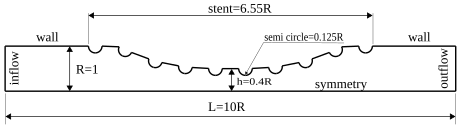
\includegraphics[scale=0.6]{./figure/CurvedStrut.png}\\
     (a) Curved Channel
     \end{center}
     \label{geometry}
     \caption{
Nondimensional domains for the dynamics analysis of 
concentration diffusion in coronary artery with drug-eluting stent. 
The lumen dimensionless width used was R = 1 and 
the lumen length was L = 10 R. The
drug-eluting stent of length equal to 6.55 R was modeled 
by 10 uniform spaced semi-circles with radius
equal to 0.125 R. An atherosclerosis was considered, 
where a sinusoidal equation was used to model 40\% of
channel obstruction.
}
\end{figure}



\section{PRELIMINARY CONCLUSION}
In this work, a numerial code for Navier-Stokes equation according to 
with species
transport equation was developed using an FE approach.
The semi-Lagrangian scheme was used to discretized the material derivative
using first order backward difference scheme and the numerical oscillations
were not seen for moderate to high Schmidt number.

\smallskip
%The dynamics of blood flow was shown to a coronary artery with atherosclerosis and
%drug-eluting stent placed.
%It is possible to observe in the Fig. \ref{conc field curved stent sc 10}  that
%the concentration field
%is more dispersed at the end of the curved channel due to
%the sense of the blood flow. It is possible that the
%drug concentration diffused affects the density and viscosity of the blood
%and consequently the Reynolds number. Thefore, the velocity field would
%also be affected. However, this influence is not considered in this work.



\section{ACKNOWLEDGEMENTS}
This optional section must be placed before the list of references.

\section{REFERENCES} 
\label{Sec:references}

\bibliographystyle{abcm}
\renewcommand{\refname}{}
\bibliography{references}



\section{RESPONSIBILITY NOTICE}
The following text, properly adapted to the number of authors, must be included in the last section of the paper:

The author(s) is (are) solely responsible for the printed material included in this paper.

\end{document}
